 %%%%%%%%%%%%%%%%%%%%%%%%%%%%% Define Article %%%%%%%%%%%%%%%%%%%%%%%%%%%%%%%%%%
\documentclass{article}
%%%%%%%%%%%%%%%%%%%%%%%%%%%%%%%%%%%%%%%%%%%%%%%%%%%%%%%%%%%%%%%%%%%%%%%%%%%%%%%

%%%%%%%%%%%%%%%%%%%%%%%%%%%%% Using Packages %%%%%%%%%%%%%%%%%%%%%%%%%%%%%%%%%%
\usepackage{geometry}
\usepackage{graphicx}
\usepackage{amssymb}
\usepackage{amsmath}
\usepackage{amsthm}
\usepackage{empheq}
\usepackage{mdframed}
\usepackage{booktabs}
\usepackage{lipsum}
\usepackage{graphicx}
\usepackage{color}
\usepackage{psfrag}
\usepackage{pgfplots}
\usepackage{bm}
\usepackage{hyperref}

\hypersetup{
    colorlinks=true,
    linkcolor=blue,
    filecolor=magenta,      
    urlcolor=cyan,
    pdfpagemode=FullScreen,
    }
%%%%%%%%%%%%%%%%%%%%%%%%%%%%%%%%%%%%%%%%%%%%%%%%%%%%%%%%%%%%%%%%%%%%%%%%%%%%%%%

% Other Settings

%%%%%%%%%%%%%%%%%%%%%%%%%% Page Setting %%%%%%%%%%%%%%%%%%%%%%%%%%%%%%%%%%%%%%%
\geometry{a4paper}

%%%%%%%%%%%%%%%%%%%%%%%%%% Define some useful colors %%%%%%%%%%%%%%%%%%%%%%%%%%
\definecolor{ocre}{RGB}{243,102,25}
\definecolor{mygray}{RGB}{243,243,244}
\definecolor{deepGreen}{RGB}{26,111,0}
\definecolor{shallowGreen}{RGB}{235,255,255}
\definecolor{deepBlue}{RGB}{61,124,222}
\definecolor{shallowBlue}{RGB}{235,249,255}
%%%%%%%%%%%%%%%%%%%%%%%%%%%%%%%%%%%%%%%%%%%%%%%%%%%%%%%%%%%%%%%%%%%%%%%%%%%%%%%

%%%%%%%%%%%%%%%%%%%%%%%%%% Define an orangebox command %%%%%%%%%%%%%%%%%%%%%%%%
\newcommand\orangebox[1]{\fcolorbox{ocre}{mygray}{\hspace{1em}#1\hspace{1em}}}
%%%%%%%%%%%%%%%%%%%%%%%%%%%%%%%%%%%%%%%%%%%%%%%%%%%%%%%%%%%%%%%%%%%%%%%%%%%%%%%

%%%%%%%%%%%%%%%%%%%%%%%%%%%% English Environments %%%%%%%%%%%%%%%%%%%%%%%%%%%%%
\newtheoremstyle{mytheoremstyle}{3pt}{3pt}{\normalfont}{0cm}{\rmfamily\bfseries}{}{1em}{{\color{black}\thmname{#1}~\thmnumber{#2}}\thmnote{\,--\,#3}}
\newtheoremstyle{myproblemstyle}{3pt}{3pt}{\normalfont}{0cm}{\rmfamily\bfseries}{}{1em}{{\color{black}\thmname{#1}~\thmnumber{#2}}\thmnote{\,--\,#3}}
\theoremstyle{mytheoremstyle}
\newmdtheoremenv[linewidth=1pt,backgroundcolor=shallowGreen,linecolor=deepGreen,leftmargin=0pt,innerleftmargin=20pt,innerrightmargin=20pt,]{theorem}{Theorem}[section]
\theoremstyle{mytheoremstyle}
\newmdtheoremenv[linewidth=1pt,backgroundcolor=shallowBlue,linecolor=deepBlue,leftmargin=0pt,innerleftmargin=20pt,innerrightmargin=20pt,]{definition}{Definition}[section]
\theoremstyle{myproblemstyle}
\newmdtheoremenv[linecolor=black,leftmargin=0pt,innerleftmargin=10pt,innerrightmargin=10pt,]{problem}{Problem}[section]
%%%%%%%%%%%%%%%%%%%%%%%%%%%%%%%%%%%%%%%%%%%%%%%%%%%%%%%%%%%%%%%%%%%%%%%%%%%%%%%

%%%%%%%%%%%%%%%%%%%%%%%%%%%%%%% Plotting Settings %%%%%%%%%%%%%%%%%%%%%%%%%%%%%
\usepgfplotslibrary{colorbrewer}
\pgfplotsset{width=8cm,compat=1.9}
\date{}
\parindent=0pt
\parskip=5pt
%%%%%%%%%%%%%%%%%%%%%%%%%%%%%%%%%%%%%%%%%%%%%%%%%%%%%%%%%%%%%%%%%%%%%%%%%%%%%%%

%%%%%%%%%%%%%%%%%%%%%%%%%%%%%%% Title & Author %%%%%%%%%%%%%%%%%%%%%%%%%%%%%%%%
\title{IMO Shortlist Writeups}
\author{Alston Yam}
%%%%%%%%%%%%%%%%%%%%%%%%%%%%%%%%%%%%%%%%%%%%%%%%%%%%%%%%%%%%%%%%%%%%%%%%%%%%%%%


\begin{document}
    \maketitle
    \section{Introduction}
    Here's a compiled list of my typed up solutions to various IMO shortlist problems during my preparation for the 66th IMO. 

    Corrections are welcome, please direct them to \url{alston.yam@gmail.com}.
    
    \section{Problems}
    \subsection{ISL 2022}

    \begin{problem}[2022 A1]
        Let $(a_n)_{n\geq 1}$ be a sequence of positive real numbers with the property that
            \[ (a_{n+1})^2 + a_na_{n+2} \leq a_n + a_{n+2} \]
        for all positive integers $n$. Show that $a_{2022}\leq 1$.
    \end{problem}

    \begin{proof}[Solution]
        Define a sequence $b_i = a_i - 1$ $\forall i$. The given condition is equivalent to \[b_nb_{n+2} + b_{n+1}(b_{n+1} + 2) \leq 0\]
        Where $b_i > -1$ $\forall i$. Now FTSOC $b_{2022} > 0$. Notice we also have \[b_{n-1}b_{n+1} + b_{n}(b_{n} + 2) \leq 0\]
        Summing the two gives
        \[b_n(b_{n-1} + b_n + 2) + b_{n+1}(b_{n+1} + b_{n-1} + 2)\leq 0\]
        Substituting $n=2022$ and $n=2021$ into the above eqeuation, we get that $b_{2021} < 0$ and also $b_{2023} < 0$ respectively. As a result, considering $n=2021$ in the first equation gives us a contradiction, and we're done.
    \end{proof}

    \pagebreak

    \subsection{ISL 2020}

    \begin{problem}[2020 A3]
        Suppose that $a,b,c,d$ are positive real numbers satisfying $(a+c)(b+d)=ac+bd$. Find the smallest possible value of
        \[ \frac{a}{b}+\frac{b}{c}+\frac{c}{d}+\frac{d}{a}. \]
    \end{problem}

    \begin{proof}
        \begin{align*}
            \frac{a}{b} + \frac{d}{c} &= \frac{ac + bd}{bc}\\
            \frac{b}{c} + \frac{a}{d} &= \frac{ac + bd}{cd}\\
            \frac{c}{d} + \frac{b}{a} &= \frac{ac + bd}{ad}\\
            \frac{d}{a} + \frac{c}{b} &= \frac{ac + bd}{ab}\\
        \end{align*}

        Summing the 4 expressions gives:

        \begin{align*}
            \left(\frac{a}{b}+\frac{b}{c}+\frac{c}{d}+\frac{d}{a}\right) + \left(\frac{b}{a}+\frac{c}{b}+\frac{d}{c}+\frac{a}{d}\right) &= (ac + bd)\left(\frac{1}{bc} + \frac{1}{cd} + \frac{1}{ad} + \frac{1}{ab}\right)\\
            &= (a+c)(b+d)\left(\frac{1}{bc} + \frac{1}{cd} + \frac{1}{ad} + \frac{1}{ab}\right)\\
            &= (ab + ad + bc + cd)\left(\frac{1}{bc} + \frac{1}{cd} + \frac{1}{ad} + \frac{1}{ab}\right)\\
            &\geq 16
        \end{align*}

        Where the last inequality is by Cauchy-Schwarz. Let $x = \frac{a}{b}, y = \frac{b}{c}, z = \frac{c}{d}, w = \frac{d}{a}$. So we have $xyzw = 1$ and
        \[(x + y + z + w) + \left(\frac{1}{x} + \frac{1}{y} + \frac{1}{z} + \frac{1}{w}\right) \geq 16\]
        \[\displaystyle\sum_{cyc}\left(x + \frac{1}{x} - 2\right) = \displaystyle\sum_{cyc}\left(\frac{{(x-1)}^2}{x}\right) = \displaystyle\sum_{cyc}x\left(1 - \frac{1}{x}\right)^2 \geq 8\]
        Finally, notice that 
        \[x + y + z + w \geq \displaystyle\sum_{cyc}x\left(1 - \frac{1}{x}\right)^2 \geq 8\]

        Finally, we can take $(a, b, c, d) = (1, 2 + \sqrt{3}, 1, 2+\sqrt{3})$ to achieve equality.
        
    \end{proof}

    \begin{problem}[2020 C2]
        In a regular 100-gon, 41 vertices are colored black and the remaining 59 vertices are colored white. Prove that there exist 24 convex quadrilaterals $Q_1, \ldots, Q_{24}$ whose corners are vertices of the 100-gon, so that
        \begin{itemize}
        \item the quadrilaterals $Q_1, \ldots, Q_{24}$ are pairwise disjoint, and
        \item every quadrilateral $Q_i$ has three corners of one color and one corner of the other color.
        \end{itemize}
    \end{problem}

    \begin{proof}
    Here's a really clever trick... We will completely ignore one of the white vertices. Now we have 41 black vertices and 58 white vertices. Notice now that no matter how we choose the quadraliterals, due to parity reasons, the number of whites unchosen is never equal to the number of blacks unchosen. 
    
    \textcolor{red}{Lemma:} 
    \end{proof}

    \begin{problem}[2020 N5]
        Determine all functions $f$ defined on the set of all positive integers and taking non-negative integer values, satisfying the three conditions:
        \begin{itemize}
        \item $(i)$ $f(n) \neq 0$ for at least one $n$;
        \item $(ii)$ $f(x y)=f(x)+f(y)$ for every positive integers $x$ and $y$;
        \item $(iii)$ there are infinitely many positive integers $n$ such that $f(k)=f(n-k)$ for all $k<n$.
        \end{itemize}
    \end{problem}

    \begin{proof}
        I claim that the answers are $f(n) = f(p)v_p(n)$ for some prime $p$. We can verify that this satisfies all 3 conditions, specifically for iii, we can pick $n$ to be all powers of $p$.

        Now we prove that these are the only set of solutions. First notice that: \[P(1, 1) \implies f(1) = f(1) + f(1) \implies f(1) = 0\]

        By condition (i) we have that there exists a prime $p$ with $f(p) > 0$. Let $p$ be the minimal such prime. Call an integer $n$ \textit{good} if $n$ satisfies condition (iii).

        \textcolor{red}{Claim 1:} If $n$ is good, then any divisor of $n$ is also good.
        Let $d'$ = $n/d$. So we have \[f(k) + f(d') = f(kd') = f(n - kd') = f(dd' - kd) = f(d'(d - k)) = f(d') + f(d-k)\]
        From which we deduce $f(d) = f(d-k)$, so $d$ is also good.

        \textcolor{red}{Claim 2:} All good numberes are of the form $n = p^km$ for some $m \leq p-1$. 
        Suppose not. Let's write a good number $n = p^k (qp + r)$. \[0 = f(r) = f(qp) = f(q) + f(p) > 0\] Which is a contradiction (second step comes from the fact that $(qp + r) \mid n$). 

        Here it's easy to see that all powers of $p$ are good, as we just take a sufficiently large $n$ with a large $p$ power. 

        \textcolor{red}{Claim 3:} For every prime $q \not= p$, we have $f(q) = 0$. 
        
        We can prove this via FLT. Write $p^{q-1} = qm + 1$, so we know that $p^{q-1}$ is good, therefore \[0 = f(1)= f(qm) = f(m) + f(q)\]
        Which is enough to imply that $f(q) = 0$.

        Now we have that $f(n) = 0$ for any $n$ coprime to $p$. So we consider an $n = p^{v_p{(n)}}m$, we have
        \[f(n) = f(m) + f(p^{v_p{(n)}}) = k\cdot v_p(n)\] for some $k$, as desired.
    \end{proof}

    \pagebreak

    \subsection{ISL 2019}

    \begin{problem}[2019 G4]
        Let $P$ be a point inside triangle $ABC$. Let $AP$ meet $BC$ at $A_1$, let $BP$ meet $CA$ at $B_1$, and let $CP$ meet $AB$ at $C_1$. Let $A_2$ be the point such that $A_1$ is the midpoint of $PA_2$, let $B_2$ be the point such that $B_1$ is the midpoint of $PB_2$, and let $C_2$ be the point such that $C_1$ is the midpoint of $PC_2$. Prove that points $A_2, B_2$, and $C_2$ cannot all lie strictly inside the circumcircle of triangle $ABC$.
    \end{problem}


    \begin{center}
        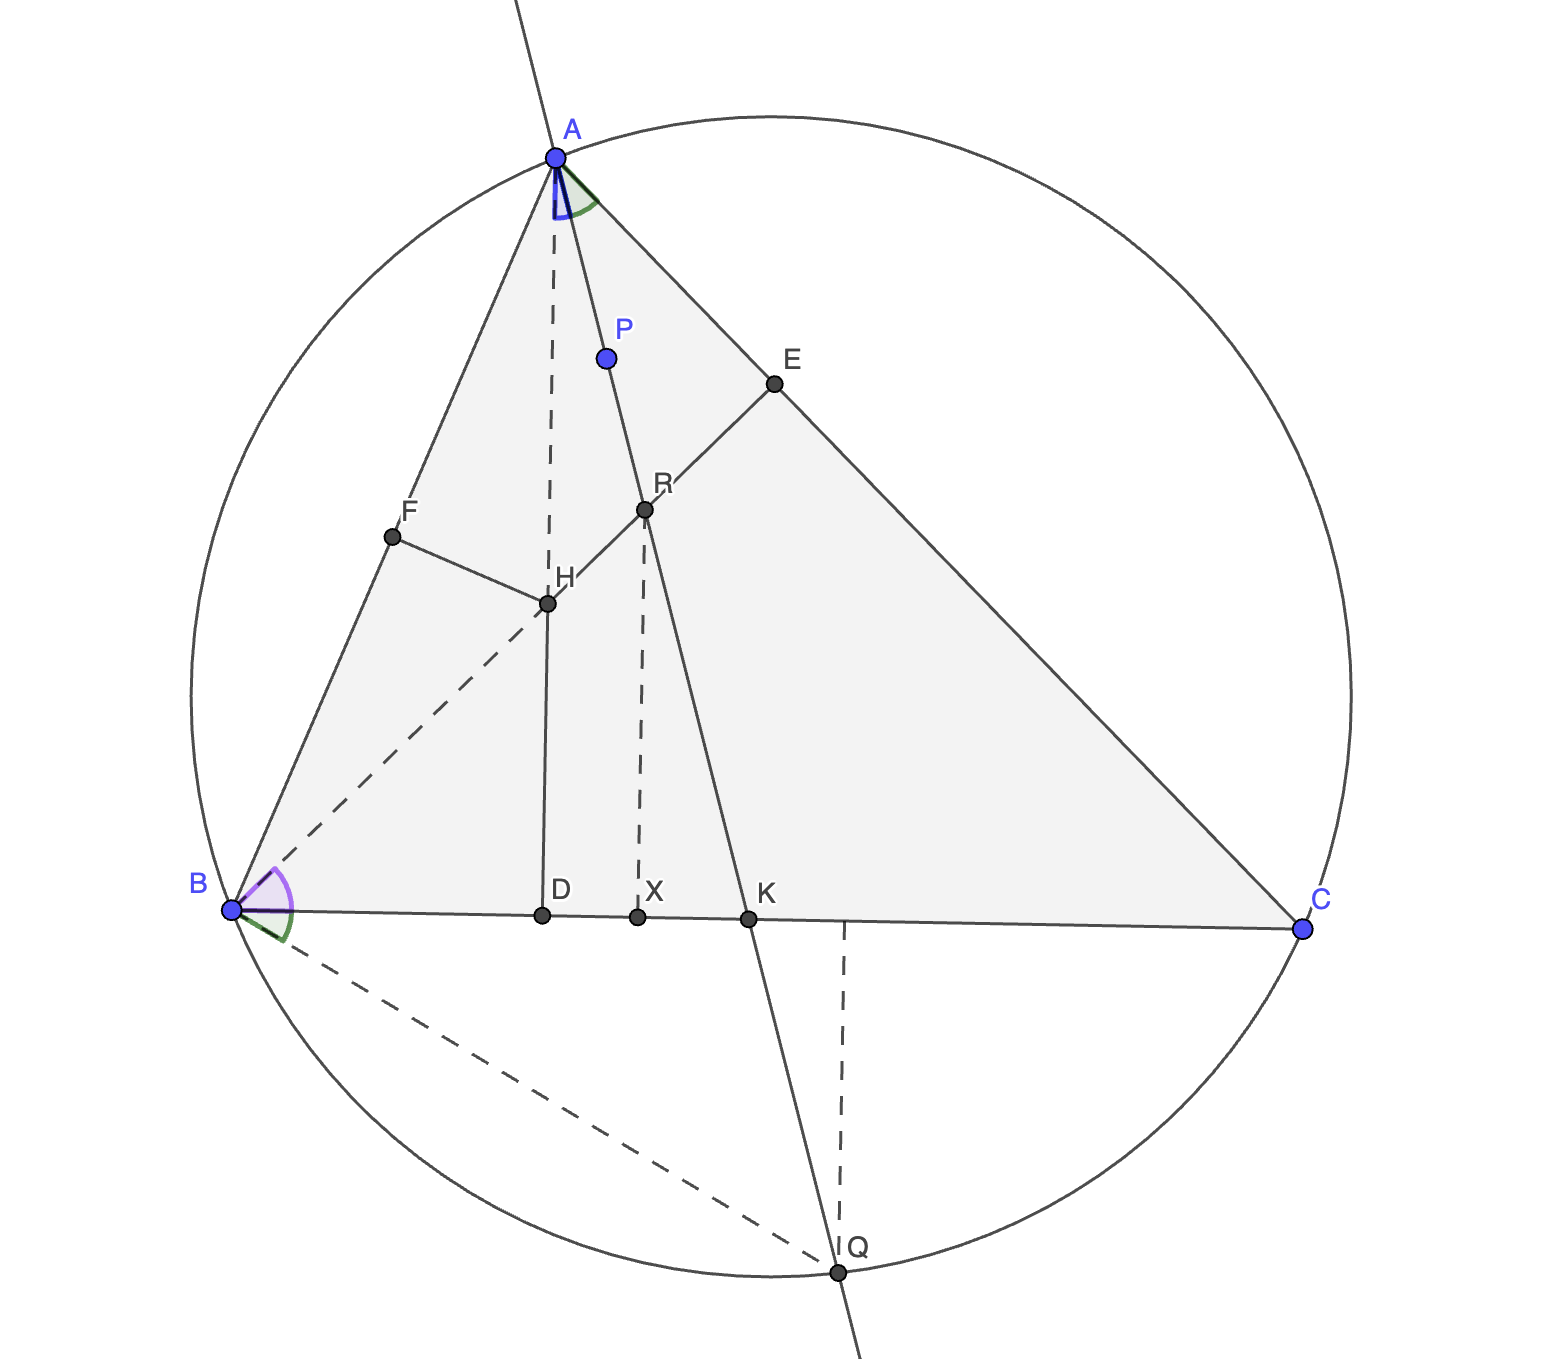
\includegraphics[scale=0.4]{2019 G4.png}

        \textit{Fig 1: Diagram for 2019 G4}
    \end{center}

    \begin{proof}
        We will first prove the case where $ABC$ is acute, and then deal with the obtuse case.

        Let $H$ denote the orthocenter of the triangle $ABC$. Drop the perpendiculars from $H$ to each of the sides $BC$, $AC$, $AB$ to be $D, E, F$ respectively. Now, WLOG point $P$ lies inside the quadrilateral $AEFH$. We will prove that the reflection of point $P$ across $K$ will be outside of $(ABC)$ (notice I have renamed a few points for convenience). In fact, we just need to prove $KR > KQ$ for this to work. 

        Now, WLOG $FH < EH$. $P$ can lie on either the same side of $AH$ as $F$, or the opposite. If $P$ lies on the same side of $AH$ as $F$, we have $KR > HD > KQ$ so we're done. Henceforth we assume $P$ lies ont he same side of $AH$ as $E$.


        In the above diagram, let 
        
        \begin{align*}
            \alpha &= \angle QBC = \angle QAC \text{ (green)}\\
            \beta &= \angle CBE = \angle DAC \text{ (purple)}\\
            \gamma &= \angle DAK \text{ (blue)}
        \end{align*}

        We start with the following manipulation:

        \begin{align*}
            \sin(2\beta)\cos(2\gamma) - \cos(2\beta)\sin(2\gamma) &< \sin(2\beta)\\
            \sin(2(\beta-\gamma)) &< \sin(2\beta)\\
            \sin(2\alpha) &< \sin(2\beta)\\
            \cos(\alpha)\sin(\alpha) &< \cos(\beta)\sin(\beta)\\
            \frac{\cos(\alpha)}{\cos(\beta)} &< \frac{\sin(\beta)}{\sin(\alpha)}
        \end{align*}

        Now, we also have by sine rule in $\triangle ARB$ and $\triangle AQB$: 
        \[\frac{BR}{\sin(\angle BAR)} = \frac{AB}{\sin(\angle ARB)} = \frac{AB}{\sin(\angle ARE)} = \frac{AB}{\sin(90-\alpha)} = \frac{AB}{\cos(\alpha)}\]
        \[\frac{BQ}{\sin(\angle BAR)} = \frac{AB}{\sin(\angle C)} = \frac{AB}{\sin(90 - \beta)} = \frac{AB}{\cos(\beta)}\]
        Hence \[\frac{BQ}{BR} = \frac{\cos(\alpha)}{\cos(\beta)} < \frac{\sin(\beta)}{\sin(\alpha)}\]

        and we have \[BQ\sin(\alpha) < BR\sin(\beta) \iff YQ < RX\]

        But this is enough to deduce $KQ < KR$ as $\triangle RKX \sim \triangle QKY$. So we're done in the $ABC$ acute case. Now we handle obtuse:

        \begin{center}
            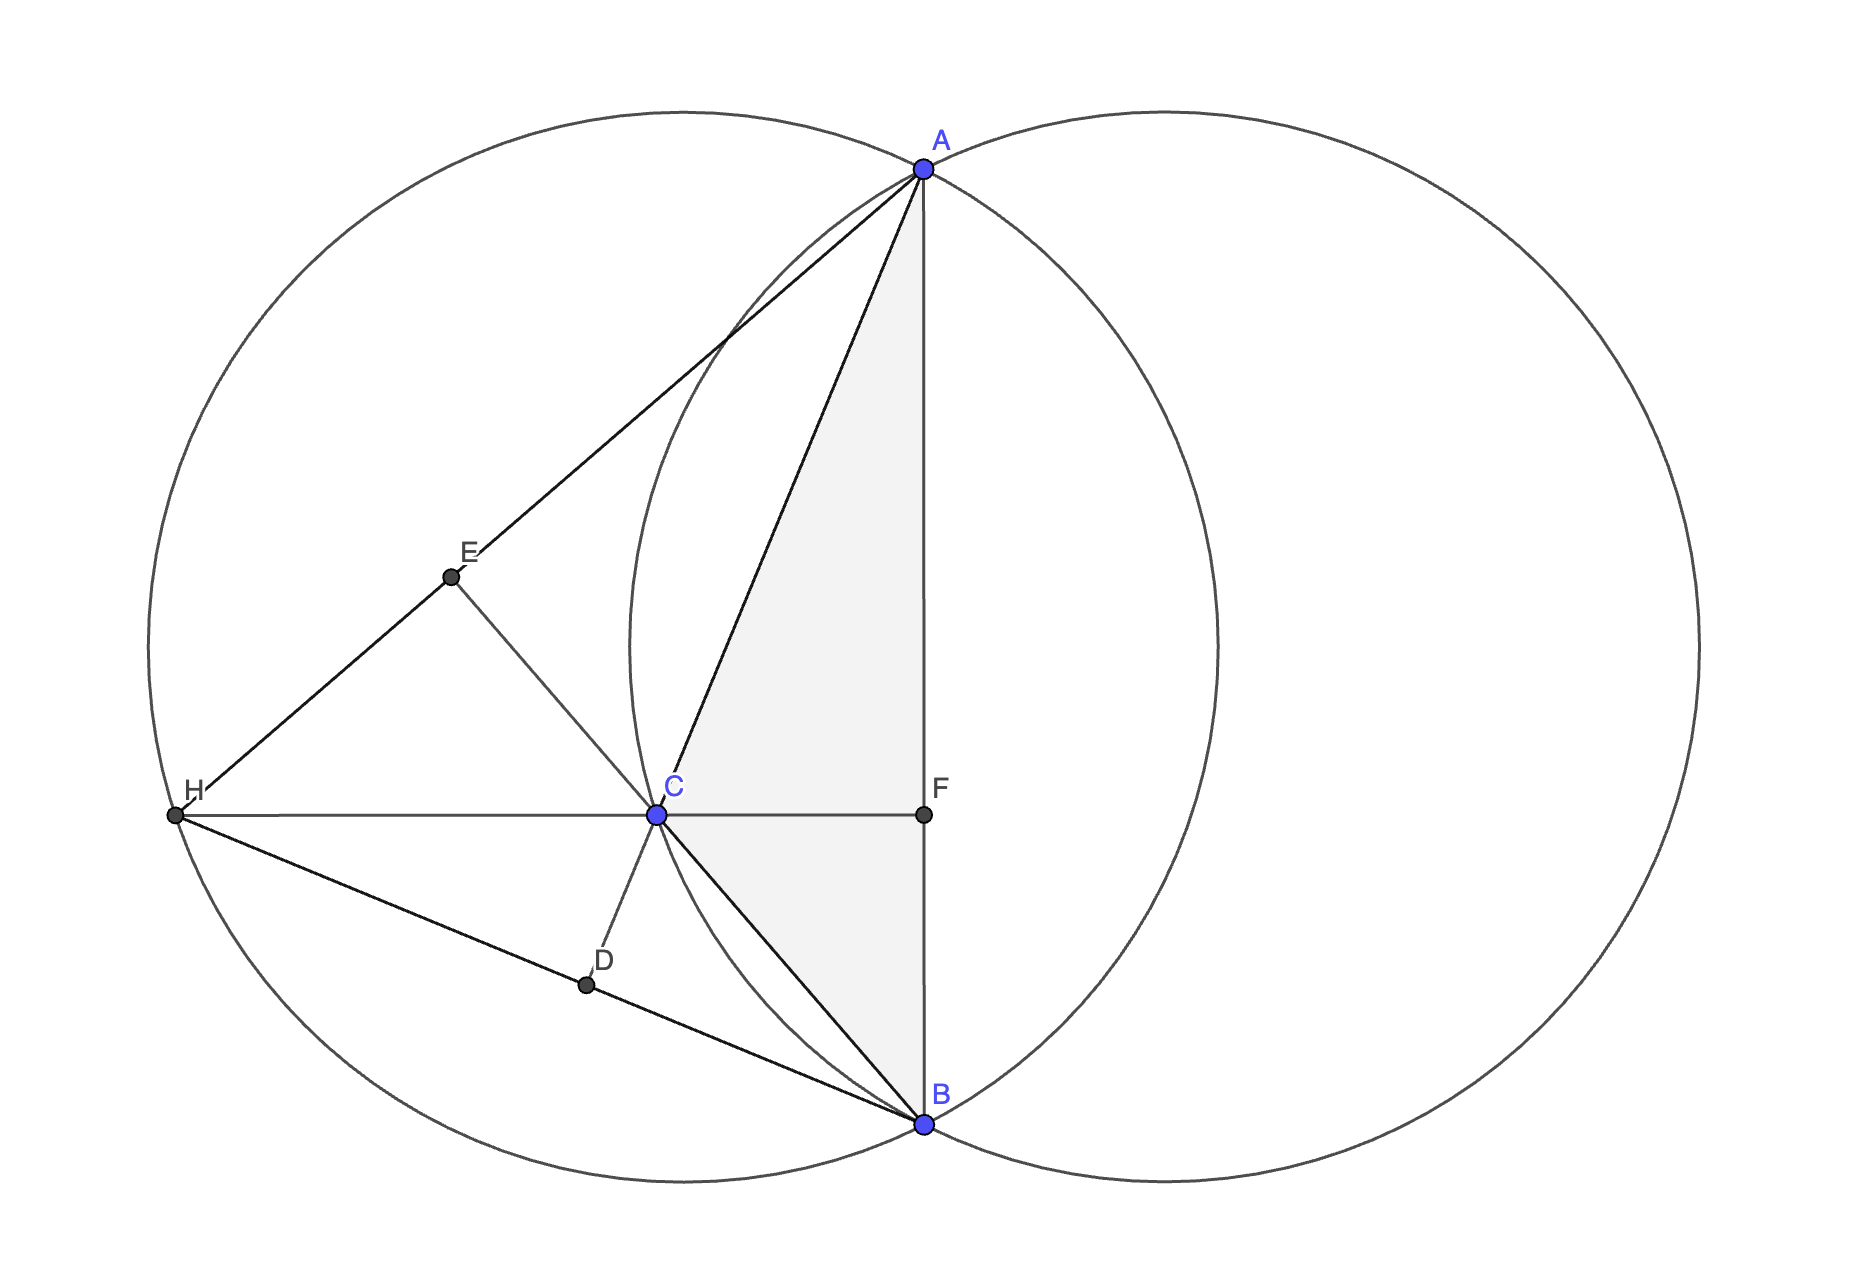
\includegraphics[scale=0.4]{2019_G4_2.png}

            \textit{Fig 2: Obtuse case of 2019 G4.}
        \end{center}


        We still construct the orthocenter $H$. Notice that $P$ must be within the shaded region, and by our work on acute triangles before, the reflection of $P$ across $BD$ or $AC$ will always lie outside of $(AHB)$, as $\triangle AHB$ is acute. Finally, notice that this is enough to finish the problem, as $(AHB)$ completely encloses the arc $ACB$ on the circumcircle of $\triangle ABC$.
    \end{proof}

    \textbf{Remark:} As I was attempting this problem, I told myself that barycentric coordinates would be an easy way to solve this, but I didn't know how they worked :( It turns out, this problem is much easier with a bary bash. 

    \begin{problem}[2019 N3]
        We say that a set $S$ of integers is \textit{rootiful} if, for any positive integer $n$ and any $a_0, a_1, \cdots, a_n \in S$, all integer roots of the polynomial $a_0+a_1x+\cdots+a_nx^n$ are also in $S$. Find all rootiful sets of integers that contain all numbers of the form $2^a - 2^b$ for positive integers $a$ and $b$.
    \end{problem}

    \begin{proof}
        I claim that the answer is $S \in \mathbb{Z}$. Clearly this works. Now we prove that if we start with the set $S = \{2^a - 2^b \mid a, b \in \mathbb{Z}^+\}$, we can then get every integer with the appropriate choices of coefficients. 
        
        First we see $1$ is in S by taking $P(x) = 2x - 2$.

        Now, notice that if $k$ is in $S$, $-k$ must also be in $S$ by taking $P(x) = x + k$. Therefore, we restrict our search to only positive integers, as the negative integers will follow.

        We will take the minimal positive integer $m$ such that $m \notin S$ and aim to find a contradiction. Let $m = 2^ep$, where $p$ is odd. Consider the number $M = 2^{e + \varphi(p) + 1} - 2^{e+1} = 2^{e+1}(2^{\varphi(p)} - 1)$. Clearly $M \in S$ and $m \mid M$ (by Euler's Theorem).
        
        We write $M = b_1m + b_2m^2 + b_3m^3 + \cdots + b_nm^n$. Then we can consider the polynomial \[P(x) = -M + b_1x + b_2x^2 + b_3x^3 + \cdots + b_nx^n\]

        This works as $b_i \in S$ $\forall i$ since $b_i < m$. Finally, notice that $m$ must be a root to the above polynomial, and so $m \in S$, and we're done.
    \end{proof}

    \pagebreak

    \subsection{ISL 2017}
    \begin{problem}[2017 A4]
        A sequence of real numbers $a_1,a_2,\ldots$ satisfies the relation
\[ a_n=-\max_{i+j=n}(a_i+a_j)\qquad\text{for all}\quad n>2017. \]
Prove that the sequence is bounded, i.e., there is a constant $M$ such that $|a_n|\leq M$ for all positive integers $n$.
    \end{problem}

    \begin{proof}

Let's denote $a_x$ to be the element with the maximum absolute value in the set $\{a_1, a_2, \cdots a_{2017}\}$. We split the problem into cases:

\textcolor{red}{Case 1}: $a_x = 0$. This case is trivial as all values in the sequence is equal to $0$.
\vspace{5pt}

\textcolor{red}{Case 2}: $a_x > 0$. Let $M = a_x$, I will prove that $-2M \leq a_i \leq M$ $\forall i$.
Proof: Notice that $$\max_{i+j=2018}(a_i+a_j) \geq a_{x} + a_{2018 - x} \geq 0$$
So $a_{2018} = -\max_{i+j=2018}(a_i+a_j) \leq 0$, i.e. It's bounded above by 0.
We also know that $$\max_{i+j=2018}(a_i+a_j) \leq M + M = 2M$$ so $a_{2018} = - \max_{i+j=2018}(a_i+a_j) \geq -2M$. So we have $$-2M \leq a_{2018} \leq 0$$
Now, if $-M \leq a_{2018} \leq 0$, we can carry on this process iteratively to get that the next element also has the bound stated above. Otherwise, assume that $-2M \leq a_{2018} < -M$. We see that $$\max_{i+j=2019}(a_i+a_j) \geq a_x + a_{2019-x} \geq M + (-2M) = -M$$
So that means $a_{2019} = -\max_{i+j=2019}(a_i+a_j) \leq M$. But also, $$\max_{i+j=2019}(a_i+a_j) \leq M + M = 2M$$
    
So we have $$-2M \leq a_{2019} \leq M$$

Thus we may continue this process iteratively to get that $-2M \leq a_i \leq M$ $\forall i$.



\textcolor{red}{Case 3}: $a_x < 0$. Let $-M = a_x$, $M > 0$. 

Notice that $$\max_{i+j=2018}(a_i+a_j) \leq 2M$$
$$\max_{i+j=2018}(a_i+a_j) \geq -2M$$

So we achieve the bound that $-2M \leq a_{2018} \leq 2M$. 


\textcolor{pink}{Case 3.1}: If $M < a_{2018} \leq 2M$, we can refer to Case 2 above to see that the sequence is bounded.

\textcolor{pink}{Case 3.2}: If $-M \leq a_{2018} \leq M$, We can iterate this process again, as $a_x = -M$ is still the $a_i$ with the largest absolute value. 


\textcolor{pink}{Case 3.3}: $-2M \leq a_{2018} < -M$.

Let $a_{2018} = -k$. Therefore there must exist $p, q$ such that $p + q = 2018$ and $a_p + a_q = k$. WLOG let $a_p \geq \frac{k}{2}$.

We see $$\max_{i+j=2019}(a_i+a_j) \geq a_p + a_{2019 - p} \geq \frac{k}{2} + (-k) = \frac{-k}{2} \geq \frac{-2M}{2} = -M$$
and also $$\max_{i+j=2019}(a_i+a_j) \leq M + M = 2M$$ So we actually see that 
$$-2M \leq a_{2019} \leq M$$

But we're done here, by considering the most negative element $a_n = -N$. There must be an $a_i$ with $a_i > \frac{N}{2}$, so the lower bound for $\max_{i+j=n}(a_i+a_j)$ is $\frac{N}{2} + (-N) = \frac{-N}{2} \geq -M$. The upper bound of $2M$ is obvious to see.

So when when calculate the next values of the sequence, the upper and lower bounds for $\max_{i+j=n}(a_i+a_j)$ are fixed at $2M$ and $-M$ respectively, so we're done.


    \end{proof}
\end{document}